% Demo Page

\chapter{Grundlagen}\label{chapter: Grundlagen}	

	\section{Abkürzungen}
	Abkürzungen im Text lassen sich mit dem Paket \textit{acronym} verwenden:\\ 
	\ac{4GDH}\\ 
	Bei der nächsten Verwendung im Text wird dann nur noch die Abkürzung verwendet \ac{4GDH}
	
	
	\section{Quellenangaben}
	Nach \cite{muhle_survey_2018} kann angenommen werden, dass ...
	
	Energie besteht aus Exergie und Anergie \cite[S. 15]{tobin_inevitable_2017}.
	
	
	\section{Abbildungen}
	In Abbildung \ref{fig: Abbildung X} ist zu erkennen, dass ... 
	\begin{figure}[ht]
		\begin{subfigure}[b]{0.49\textwidth}
			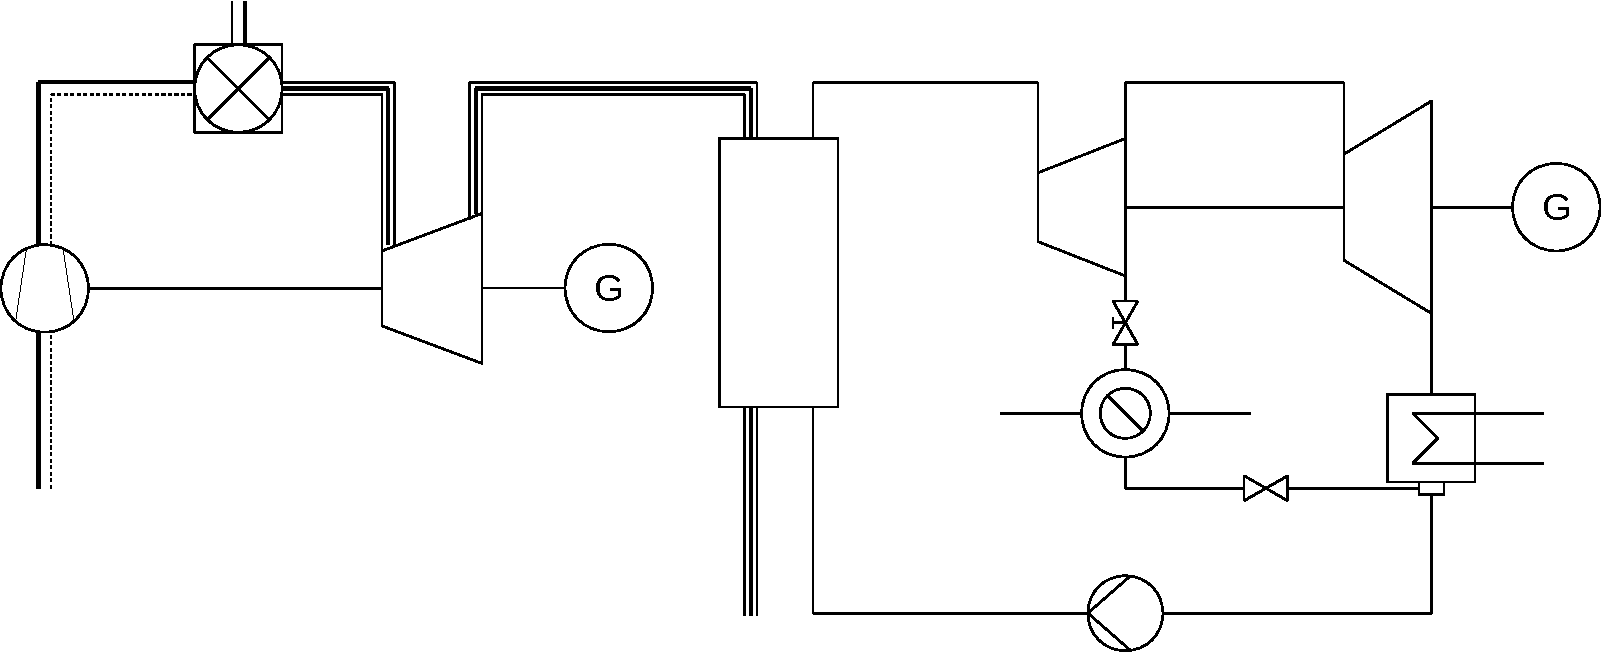
\includegraphics[width=1\textwidth]{SchaltplanGuD.pdf}
			\subcaption{Gas- und Dampfkraftwerk}
			\label{subfigure: Schaltplan_GuD}
		\end{subfigure}
		\hfill
		\begin{subfigure}[b]{0.49\textwidth}
			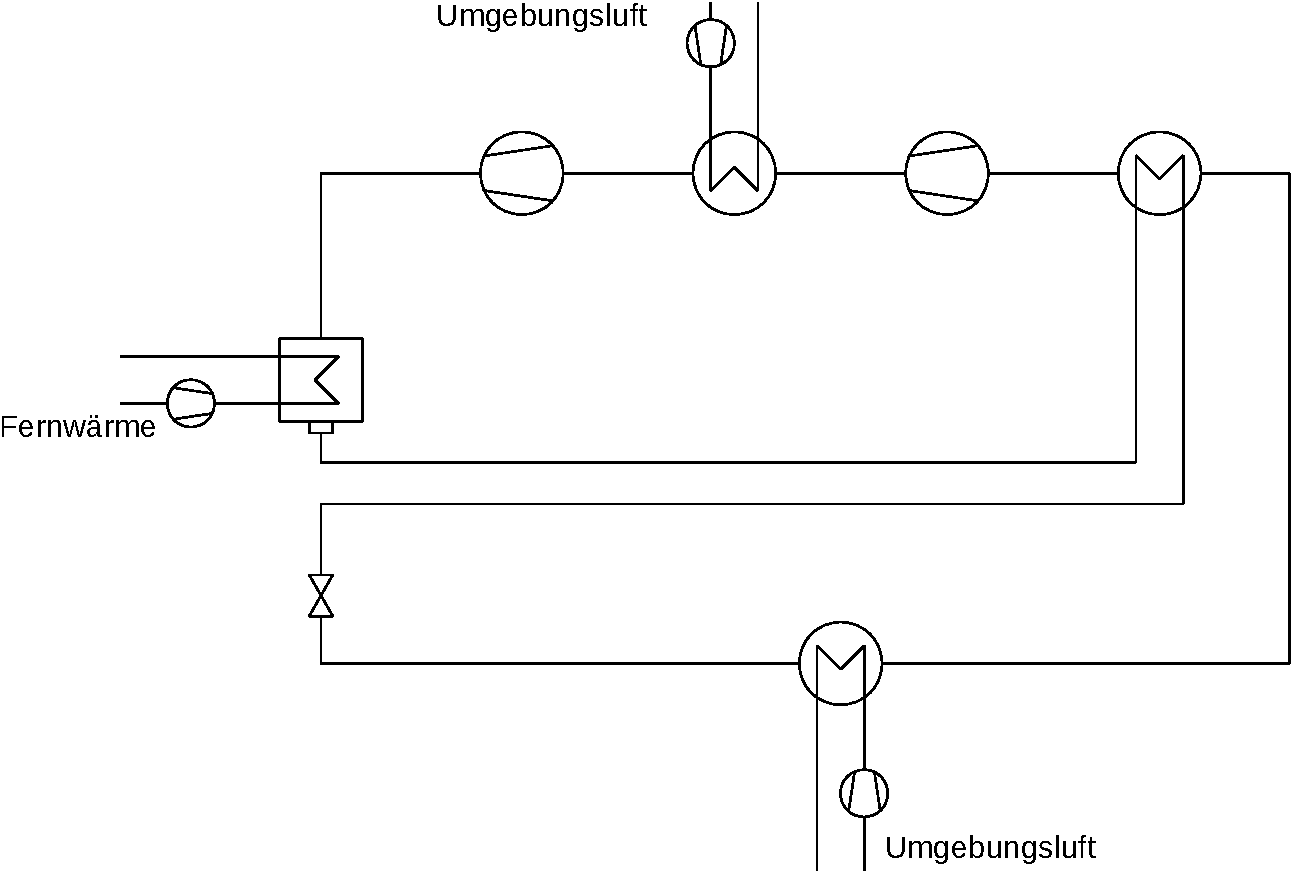
\includegraphics[width=1\textwidth]{Heatpump.pdf}
			\subcaption{Wärmepumpe}
			\label{subfigure: Schaltbild_Heatpump}
		\end{subfigure}
		\caption[Gegenüberstellung Gas- und Dampfkraftwerk mit Wärmepumpe]{Abbildung \ref{subfigure: Schaltplan_GuD} zeigt das Wärmeschaltbild eines Gas- und Dampfkraftwerks mit einer einfachen Entnahme im Dampfturbinen Teil. Abbildung \ref{subfigure: Schaltbild_Heatpump} zeigt hingegen das Schaltbild einer Kompressionswärmepumpe mit einfacher Kondensatunterkühlung.}
		\label{fig: Abbildung X}
	\end{figure}
	
	
	\section{Tabellen}
	Durch das Hinzufügen von Fußnoten innerhalb einer Tabelle können zusätzliche Informationen zu bestimmten Werten oder Bezeichnungen gegeben werden. In Tabelle \ref{tab: Nennparameter GuD} gibt die Fußnote an, dass die angegebene Grädigkeit für alle Wärmeübertrager gleichermaßen gilt.
	
    	\begin{center}
    	    \captionof{table}{Auslegungsparameter des Gas- und Dampfkraftwerks}
    		\begin{threeparttable}
        		\begin{tabular}{lllll}
        			\hline 
        			Teilprozess & Parameter  & Symbol  & Einheit  & Wert\tabularnewline
        			\hline 
        			\textbf{Fernwärme} & Vorlauftemperatur  & $T_{\text{VL}}$  & \textdegree C  &  124\tabularnewline
        			& Rücklauftemperatur  & $T_{\text{RL}}$  & \textdegree C  & 50\tabularnewline
        			& Druck  & $p_{\text{FW}}$  & bar  & 10\tabularnewline
        			& Wärmeaufnahme & $\dot{Q}_\text{DH}$ & MW & 145 \tabularnewline
        			\textbf{Gasturbinenprozess} & Brennstoffmassenstrom  & $\dot{m}_{\text{Fuel}}$  & kg/s  & 11,58 \tabularnewline
        			& Umgebungstemperatur  & $T_{\text{U}}$  & \textdegree C & 20 \tabularnewline
        			& Verbrennunstemperatur  & $T_{\text{CC}}$  & \textdegree C & 1500 \tabularnewline
        			& Abgastemperatur  & $T_{\text{AG}}$  & \textdegree C & 150 \tabularnewline
        			& Verdichterdruckverhältnis  & pr  & - & 14 \tabularnewline
        			& Verdichterwirkungsgrad  & $\eta_{\text{V}}$  & - & 0,91 \tabularnewline
        			& Gasturbinenwirkungsgrad  & $\eta_{\text{GT}}$  & - & 0,9 \tabularnewline
        			\textbf{Dampfturbinenprozess} & Frischdampftemperatur  & $T_{\text{FD}}$  & \textdegree C & 600 \tabularnewline
        			& Frischdampfdruck  & $p_{\text{FD}}$  & bar & 100 \tabularnewline
        			& Entnahmedruck  & $p_{\text{E}}$  & bar & 3 \tabularnewline
        			& Abdampfdruck  & $p_{\text{AD}}$  & bar & 0,04 \tabularnewline
        			& Dampfturbinenwirkungsgrad  & $\eta_{\text{DT}}$  & - & 0,9 \tabularnewline
        			& Pumpenwirkungsgrad  & $\eta_{\text{P}}$  & - & 0,8 \tabularnewline
        			& Grädigkeit\tnote{1}  & $\Delta T$  & K & 5 \tabularnewline
        			\hline 
        		\end{tabular}
    
    		\begin{tablenotes}\footnotesize 
    			\item[1] Grädigkeit wird für alle verwendeten Wärmeübertrager gleich angenommen.
    		\end{tablenotes}
    	\end{threeparttable}
    	\label{tab: Nennparameter GuD}
	\end{center} 

    \section{Code}
        Die Darstellung von Code erfolgt über das Paket \textit{listings}. Einstellung dazu sind in der Präambel zu finden. Ein Beispiel für Code in \LaTeX:
        \begin{lstlisting}[language=python,numbers=none]
import numpy as np

def pi(n):
    t = 0
    for i in range(n):
        x = np.random.rand()
        y = np.random.rand()
        
        if np.sqrt(x**2 + y**2) <= 1:
            t += 1
    return 4 * (t / n)
\end{lstlisting}   
